\chapter{Модальные регулятор}
\label{ch:chap1}
\section{Условие задачи}

Необходимо рассмотреть систему:
$$
  \dot{x} = Ax + Bu
$$ и выполнить следующие шаги:

\begin{itemize}
\item   Найти собственные числа матрицы $A$ и определить управляемость каждого из них. 
Сделать вывод об управляемости и стабилизируемости системы.
\item Построить схему моделирования системы, замкнутой регулятором $u = Kx$.
\item Рассмотреть предложенные желаемые спектры замкнутой системы $(A+BK)$ и определить, 
какие из них достижимы, а какие нет. Обосновать выбор.
\item Для каждого из достижимых спектров вашего варианта:
  \begin{itemize}
    \item Найти соответствующую матрицу регулятора $K$, приводящий спектр 
    замкнутой системы к желаемому.
    \item Определить собственные числа матрицы замкнутой системы $(A+BK)$ и 
    сравнить с желаемым спектром в подтверждение корректности синтеза регулятора.
    \item  Выполнить компьютерное моделирование и построить графики формируемого 
    регулятором управления $u(t)$ и вектора состояния замкнутой системы $x(t)$
     при начальных условиях $x(0) = \begin{bmatrix} 1 & 1 & 1 \end{bmatrix}^T$.
  \end{itemize}
\item Сопоставить полученные результаты компьютерного моделирования для рассмотренных спектров, 
оценить возможные сравнительные преимущества и недостатки  каждого из них.
\end{itemize}

\section{Решение задачи}

Параметры для объекта:
$$
  A = \begin{bmatrix}
  12 & -1 & 14 \\
  6 & 0 & 6 \\
  -6 & -2 & -8 
  \end{bmatrix} \tab
  B = \begin{bmatrix}
    11 \\ 7 \\ -7 
  \end{bmatrix}
$$

\subsection{Исследование управляемости системы}

Найдём собственные числа матрицы $A$:
$$
    \lambda_{1,2} = 3 \pm 3i, \tab \lambda_3 = -2
$$

Вычислим матрицу Хаутуса для каждого собственного числа:
$$
    H_1 = \begin{bmatrix}
          A - \lambda_1 I & B   
          \end{bmatrix} = 
    \begin{bmatrix}
    9-3i & -1 & 14 & 11 \\  
    6 & -3-3i & 6 & 7 \\  
    -6 & -2 & -11 -3i & -7   
    \end{bmatrix}
$$
$$
rank(H_1) = 3
$$
Значит собственное число $\lambda_1$ является управляемым, если ранг его матрицы Хаутуса равняется порядку системы.
$$
    H_2 = \begin{bmatrix}
          A - \lambda_2 I & B   
          \end{bmatrix} = 
    \begin{bmatrix}
      9+3i & -1 & 14 & 11 \\  
      6 & -3+3i & 6 & 7 \\  
      -6 & -2 & -11+3i & -7   
    \end{bmatrix}
$$
$$
rank(H_2) = 3
$$
Аналогично, собственное число $\lambda_2$ является управляемым.
$$
    H_3 = \begin{bmatrix}
          A - \lambda_3 I & B   
          \end{bmatrix} = 
    \begin{bmatrix}
      14 & -1 & 14 & 11 \\
      6 & 2 & 4 & 7 \\
      -6 & -2 & -4 & -7
    \end{bmatrix}
$$
$$
$$
$$
rank(H_3) = 2
$$
Последнее собственное число $\lambda_3$ уже не управляемое. Значит система по критерию Хаутуса будет не полностью управляемой. 

Однако система будет стабилизируемой, потому что это все неустойчивые (их нет) собственные числа у нас будут управляемые.

\subsection{Достижимые спектры}
Нам дан следующий набор спектров замкнутной системы $(A+BK)$:
$$
  \begin{aligned}
    \sigma_1 = \{-1, -1, -1\} \\
    \sigma_2 = \{-2, -2, -2\} \\
    \sigma_3 = \{-1, -10, -100\} \\
    \sigma_4 = \{-2, -20, -200\} \\
    \sigma_5 = \{-1, -1-3i, -1+3i\} \\
    \sigma_6 = \{-2, -2-6i, -2+6i\} 
  \end{aligned}
$$

Из него не все спектры мы сможем использовать как достижимы у матрицы замкнутой $(A+BK)$ на регулятор системы, потому что наша система не полностью управляема.
Ограничивает нас $\lambda_3=-2$ (не управляемое собственное число), которое нельзя будет изменить никак с помощью регулятора, поэтому оно обязано остаться одним из собственных чисел $(A+BK)$ после замыкания.
После такого отбора останутся следующие спектры, и они уже будут достижимыми:

$$
  \begin{aligned}
    \sigma_2 = \{-2, -2, -2\} \\
    \sigma_4 = \{-2, -20, -200\} \\
    \sigma_6 = \{-2, -2-6i, -2+6i\} 
  \end{aligned}
$$

\subsection{Первый спектр}
$$
    \sigma_1 = \{-2, -2, -2\} \\
$$

Найдём матрицу регулятора K, приводящий спектр замкнутой системы к желаемому. Для её получения воспользуемся следующей системой:
$$
\begin{cases}
  AP - PG = BY, \\
  K = -YP^{-1}
\end{cases}
$$ и убедимся в том, что следующие условия также более-менее выполняются:
$$
  \begin{cases}
    \sigma(A) \cap \sigma(G) = \emptyset, \\
    (A,B) - \text{управляема, то всегда будет существовать } P \\
    (Y,G) - \text{ наблюдаема } 
  \end{cases}
$$
Матрицы $G,Y$ - выборочные и вспомогательные при синтезе регулятора:
\begin{itemize}
  \item Выбираем $G\in\mathbb{R}^{n\times n}$ с желаемым спектром $\sigma(G)$
  \item Выбираем $Y\in\mathbb{R}^{m\times n}$ такую, чтобы пара $(Y, G)$ была наблюдаема
  \item Ищем $P\in\mathbb{R}^{n\times n}$ как решение уравнения Сильвестра $AP - PG = BY$
  \item Вычисляем коэффициенты регулятора: $K = -YP^{-1}$
\end{itemize}

В нашем случае пара $(A,B)$ - лишь стабилизируема, но это не значит, что регулятор нельзя синтезировать, пока что это лишь значит, что
решение может быть не единственным или/и вырожденным. Остальные два условия мы выполним умным выбором $Y,G$:
$$
G = \begin{bmatrix}
    -2  &  1  & 0 \\
     0  & -2  & 1 \\
     0  &  0  & -2 
\end{bmatrix} \tab Y = \begin{bmatrix}
  1 & 1 & 1
\end{bmatrix}
$$

Проделав вычисления, получим следующие коэффициенты:
$$
  K = \begin{bmatrix}
    1.09 & -2.08 & 1.06
  \end{bmatrix}
$$
Тогда получим следующие собственные числа $(A+BK)$:
$$
    \lambda_{1,2,3} = -2
$$
Что совпадает с исходно заданным спектром, а значит контроллер мы синтезировали верно.

Для проведения моделирования была составлена следующая схема:
\begin{figure}[ht]
  \centering
  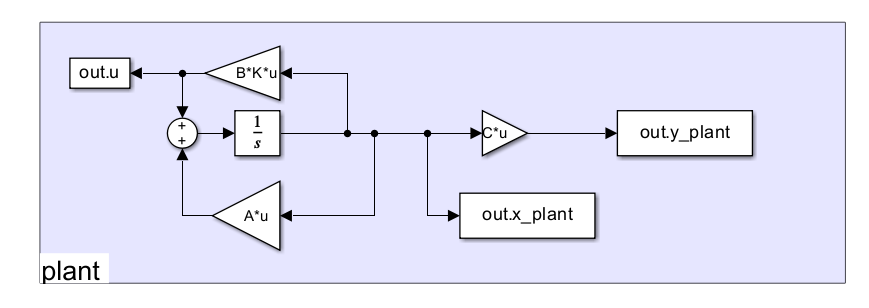
\includegraphics[width=1.0\textwidth]{model_controller.png}
  \caption{Модель с модальным регулятором}
\end{figure}

С помощью неё построим графики управления $u(t)$ от регулятора и вектора состояния замкнутой системы $x(t)$
при начальных условиях $x(0) = \begin{bmatrix} 1 & 1 & 1 \end{bmatrix}^T$:
\newpage
\begin{figure}[ht]
  \centering
  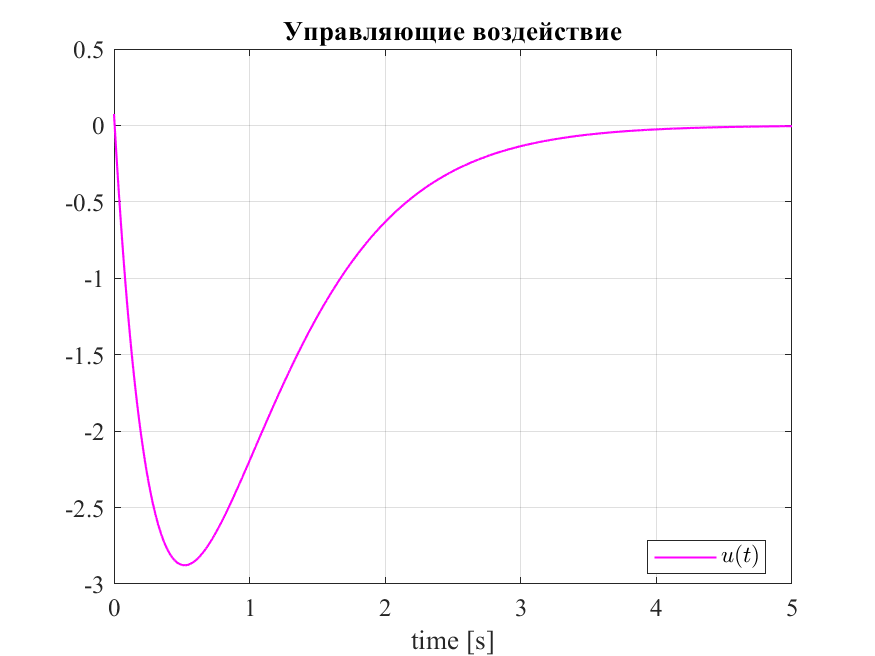
\includegraphics[width=0.8\textwidth]{ctrl_u1.png}
  \caption{Сигнал управления}
\end{figure}
\begin{figure}[ht]
  \centering
  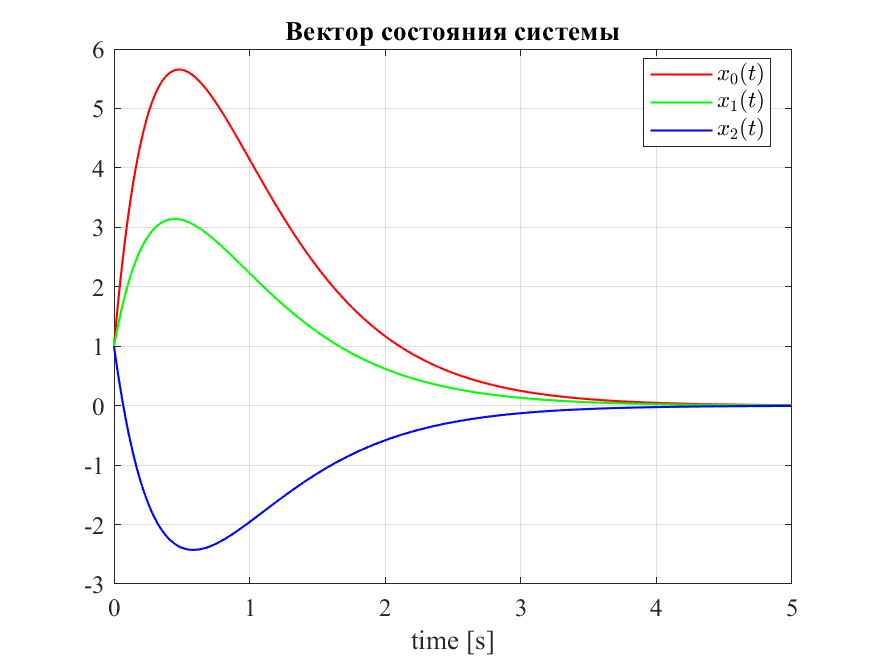
\includegraphics[width=0.8\textwidth]{ctrl_x1.png}
  \caption{Состояние системы}
\end{figure}

\newpage
\subsection{Второй спектр}
$$
    \sigma_2 = \{-2, -20, -200\} \\
$$

Найдём матрицу регулятора K, воспользуемся следующей системой:
$$
\begin{cases}
  AP - PG = BY, \\
  K = -YP^{-1}
\end{cases}
$$ Для этого с умом выберем $Y,G$:
$$
G = \begin{bmatrix}
    -2  &  0  & 0 \\
     0  & -20  & 0 \\
     0  &  0  & -200 
\end{bmatrix} \tab Y = \begin{bmatrix}
  1 & 1 & 2
\end{bmatrix}
$$

Проделав вычисления, получим следующие коэффициенты:
$$
  K = \begin{bmatrix}
    425.89 & -387.02 & 314.51
  \end{bmatrix}
$$
Тогда получим следующие собственные числа $(A+BK)$:
$$
    \lambda_1 = -2, \tab \lambda_2 = -20, \tab \lambda_3 = -200
$$
Что совпадает с исходно заданным спектром, а значит контроллер мы синтезировали верно.

Построим графики управления $u(t)$  и вектора состояния $x(t)$:
\begin{figure}[ht]
  \centering
  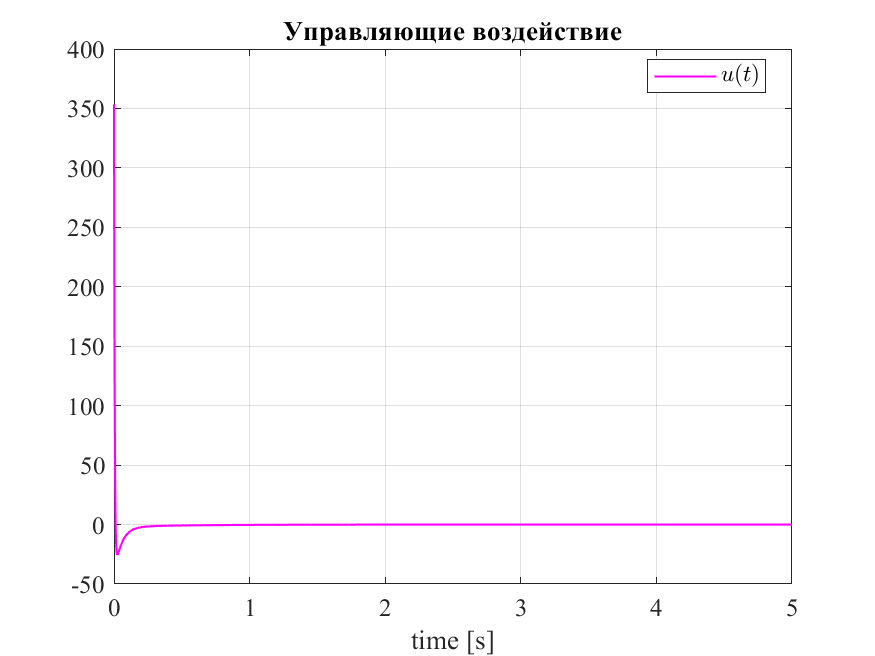
\includegraphics[width=0.8\textwidth]{ctrl_u2.png}
  \caption{Сигнал управления}
\end{figure}
\begin{figure}[ht]
  \centering
  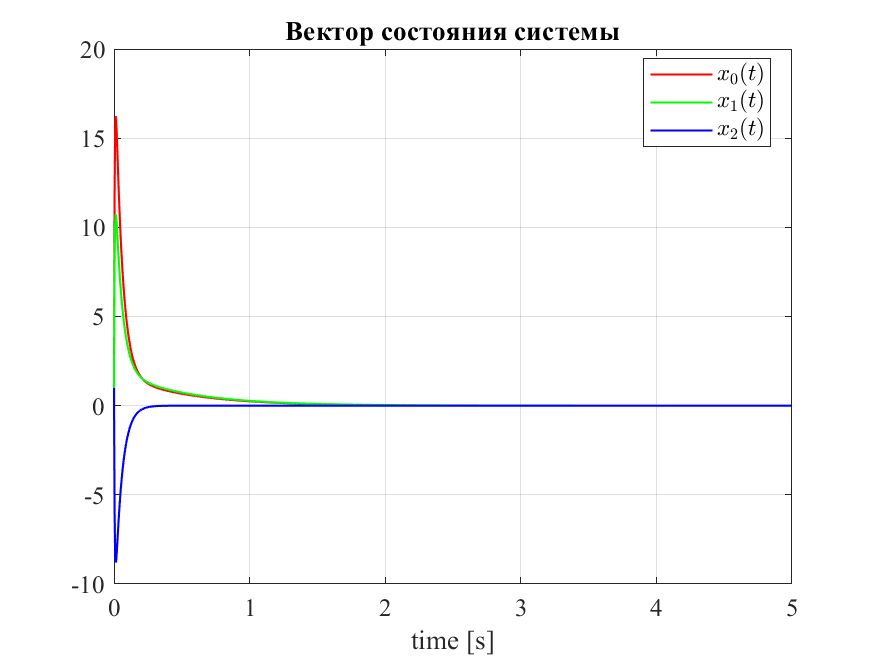
\includegraphics[width=0.8\textwidth]{ctrl_x2.png}
  \caption{Состояние системы}
\end{figure}

\newpage
\subsection{Третий спектр}
$$
  \sigma_3 = \{-2, -2-6i, -2+6i\} 
$$

Найдём матрицу регулятора K, воспользуемся следующей системой:
$$
\begin{cases}
  AP - PG = BY, \\
  K = -YP^{-1}
\end{cases}
$$ Для этого с умом выберем $Y,G$:
$$
G = \begin{bmatrix}
    -2  &  0  & 0 \\
     0  & -2  & 6 \\
     0  &  -6  & -2 
\end{bmatrix} \tab Y = \begin{bmatrix}
  1 & 1 & 0
\end{bmatrix}
$$

Проделав вычисления, получим следующие коэффициенты:
$$
  K = \begin{bmatrix}
    4.45 & -5.09 & 3.32
  \end{bmatrix}
$$
Тогда получим следующие собственные числа $(A+BK)$:
$$
    \lambda_1 = -2, \tab \lambda_{2,3} = -2 \pm 6i
$$
Что совпадает с исходно заданным спектром, а значит контроллер мы синтезировали верно.

Построим графики управления $u(t)$  и вектора состояния $x(t)$:
\newpage
\begin{figure}[ht]
  \centering
  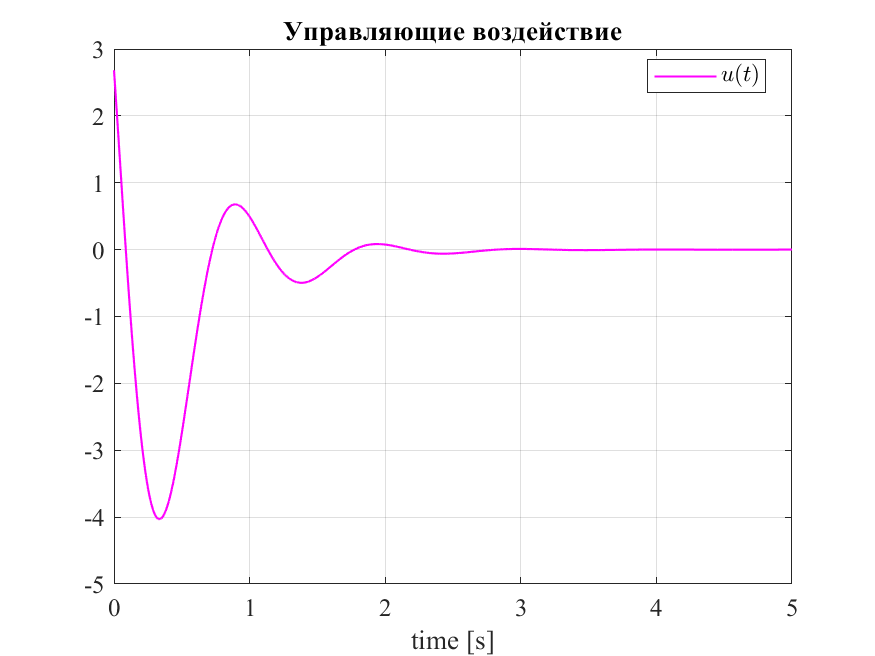
\includegraphics[width=0.8\textwidth]{ctrl_u3.png}
  \caption{Сигнал управления}
\end{figure}
\begin{figure}[ht]
  \centering
  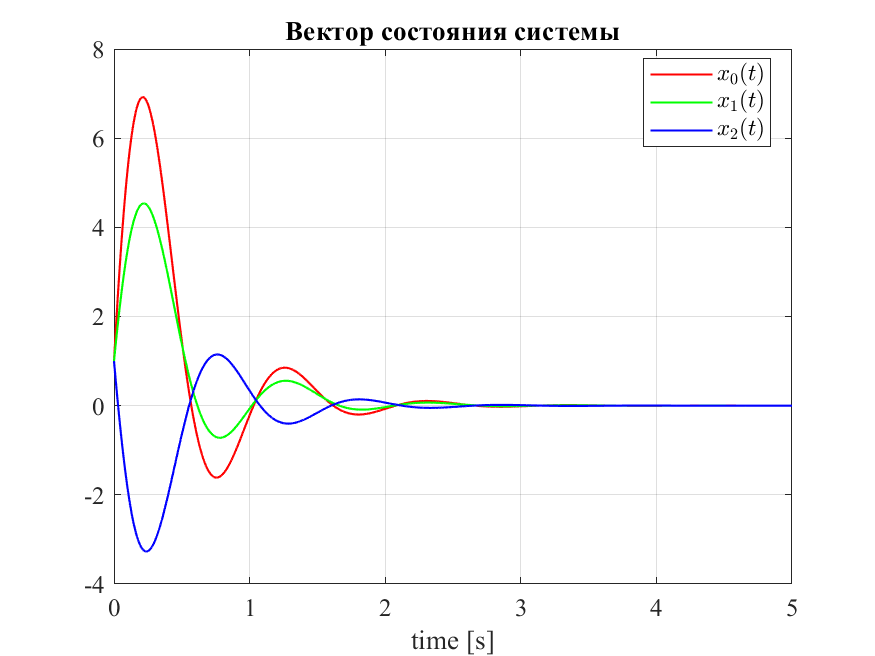
\includegraphics[width=0.8\textwidth]{ctrl_x3.png}
  \caption{Состояние системы}
\end{figure}

\subsection{Сравнение выбора собственных чисел для синтеза регулятора}

В первом случае мы выбрали относительно небольшие устойчивые моды, поэтому регулятор в целом корректировал систему плавно и с небольшим переругулированием.

Во втором случае мы решили ускорить процесс управления и многократно увеличили моды, поэтому управление действовало аггресивно, но привело
систему в нулевую позицию очень быстро. Однако в реальном мире таким управлением воспользоваться вряд ли удастся - нам помешают физические ограничения по току, 
потому иначе просто двигатель сможет сгореть от такого резкого и высокого напряжения, или просто такое управление переполнит буфер памяти контроллера. В общем, такое управление довольно рисковано.

В треьем случае в спектр вошла комплексно сопряжённая мода, поэтому система сходится с небольшими колебаниями, но вполне плавно, с небольшим перерегулированием, потому что вещественная часть этих мод не слишком велика.




\subsection{Вывод}

Исследование системы задания показало, что стабилизируемой системой мы можем управлять с разным "характером" сходимости, и не важна, что она не полностью управляема. 
Для управления мы успешно синтезировали модальный регулятор с помощью уравнения Сильвестра, желаемые спектры и спектр матрицы $(A+BK)$ - сошлись, что свидетельствует о корректном синтезе.

\endinput